
\documentclass[template=tabling,81pt,headonall]{azmoon}
\usepackage{xepersian}
\usepackage{amsfonts}
\usepackage{graphicx}
\usepackage{svg}
\svgpath{ {./images/} }
\graphicspath{ {./images/} }
\settextfont{Yas}
\setdigitfont{A Iranian Sans}
\usepackage{fontawesome5}

\printanswers
    \teacher{محمد صالح علی اکبری}
    \teachertitle{دبیر}
    \city{گناباد}
    \schooltitle{متوسطه دوره اول}
    \school{هنرستان خوارزمی}
    \grade{دهم}
    \branch{101}
    \topic{ریاضی}
    \examdate{۲۱/۱۲/۱۴۰۳}
    \answertime{۵۰ دقیقه}
    \begin{document}
	\begin{questions}
		\nointerlineskip%
		\vskip-\baselineskip
		\question[1]{%
قرینه عدد 5 چند است؟
    \begin{fourchoice}[4]\choice{$5$}
\choice{$-5$}
\choice{$-\dfrac{1}{5}$}
\choice{$\dfrac{1}{5}$}
\end{fourchoice}

            }\question[1]{%
حاصل عبارت $\dfrac{4 - \sqrt{36-11}}{2} = $ کدام است؟
    \begin{fourchoice}[4]\choice{$-3$}
\choice{$5$}
\choice{$-\dfrac{1}{2}$}
\choice{$\dfrac{1}{2}$}
\end{fourchoice}

            }\question[1]{%
حاصل عبارت $\dfrac{6 + 4}{2} = $ کدام است؟
    \begin{fourchoice}[4]\choice{$5$}
\choice{$8$}
\choice{$7$}
\choice{$10$}
\end{fourchoice}

            }\question[1]{%
نمودار زیر محل تقاطع دو نمودار $y_1 = -2x$ و $y_2 = -x^2$ جواب معادله $-2x = -x^2$ چند است؟ \\ 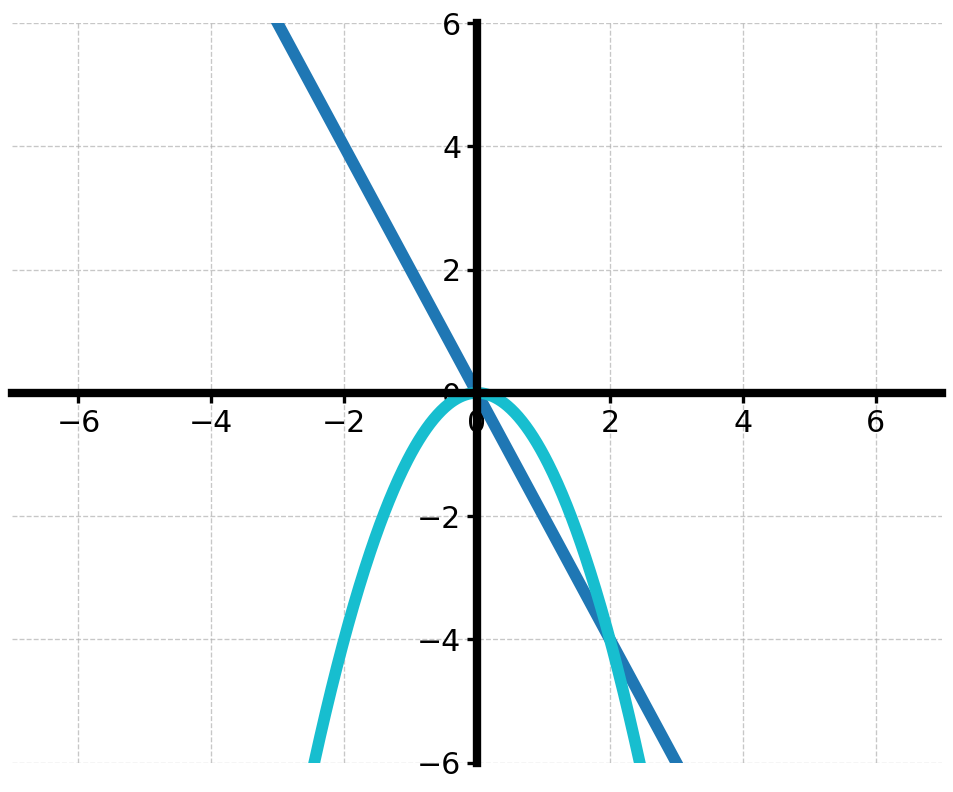
\includegraphics[scale = 0.6]{y__=___-_2x_and_y__=___-_1x_power_2}
    \begin{fourchoice}[4]\choice{$1$}
\choice{$-4$}
\choice{$3$ و $-1$}
\choice{$2$ و $0$}
\end{fourchoice}

            }\question[1]{%
نمودار زیر محل تقاطع دو نمودار $y_1 = -\dfrac{1}{4}x+2$ و $y_2 = -\dfrac{1}{4}x^2+\dfrac{3}{4}x+4$ جواب معادله $-\dfrac{1}{4}x+2 = -\dfrac{1}{4}x^2+\dfrac{3}{4}x+4$ چند است؟ 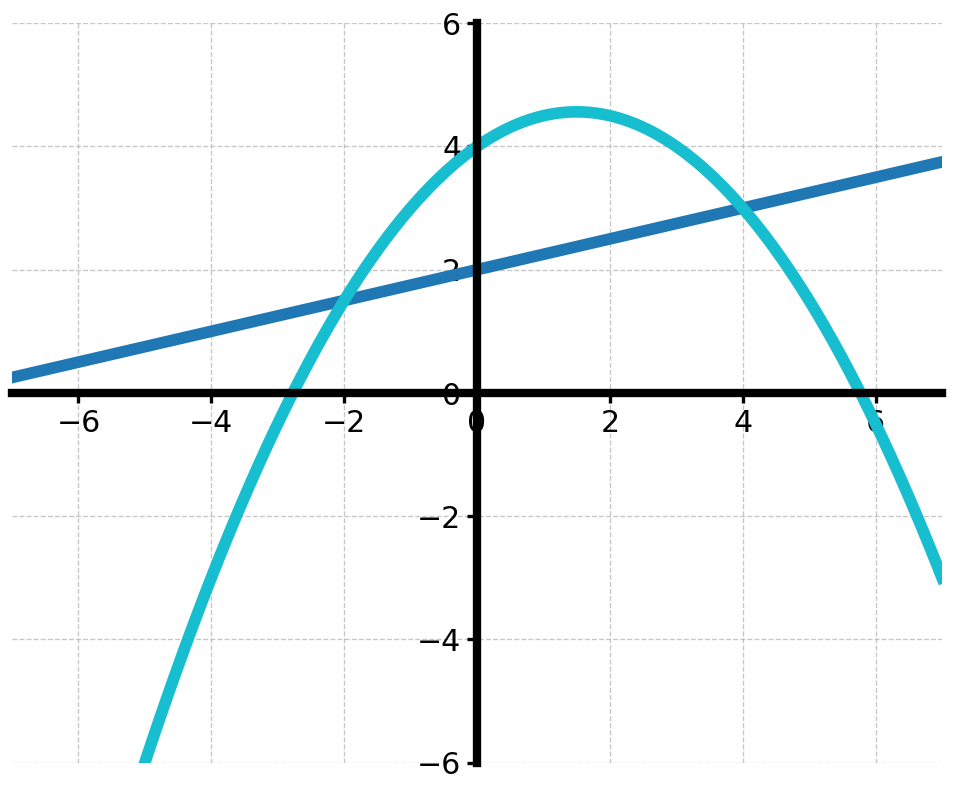
\includegraphics[scale = 0.4]{y__=___+_0.25x_+_2_and_y__=___-_0.25x_power_2__+_0.75x__+_4}
    \begin{fourchoice}[4]\choice{$3$}
\choice{$-3$}
\choice{$4$ و $-2$}
\choice{$-4$ و $2$}
\end{fourchoice}

            }\question[1]{%
برای حل معادله $x^2 + 3x - 4 = 0$ آن را به کدام یک از عبارت‌های زیر می‌توان تبدیل کرد؟ (در حال حل معادله به روش هندسی هستیم)
    \begin{fourchoice}[4]\choice{$x^2 = +3x + 4$}
\choice{$x^2 = +3x - 4$}
\choice{$x^2 = -3x + 4$}
\choice{$x^2 = -3x - 4$}
\end{fourchoice}

            }\question[1]{%
کدام تصویر مربوط به حل معادله به روش هندسی معادل $3x^2 + x - 6 = 0$ است؟
    \begin{fourchoice}[2]\choice{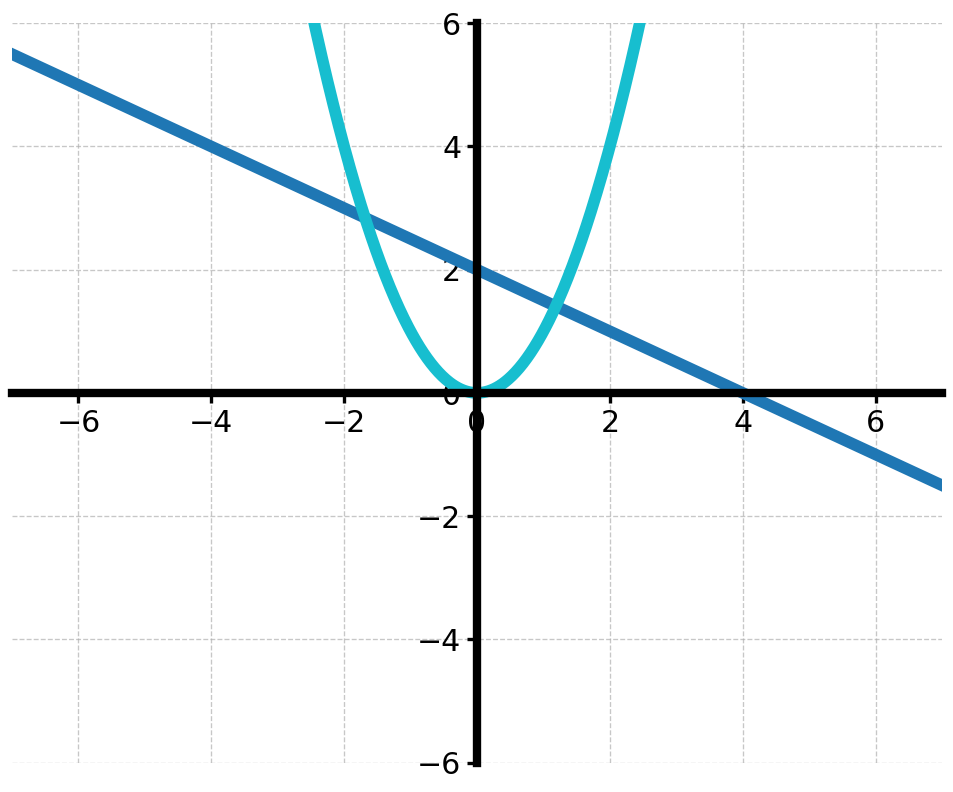
\includegraphics[scale = 0.35]{y__=___-_0.5x_+_2_and_y__=__x_power_2}}
\choice{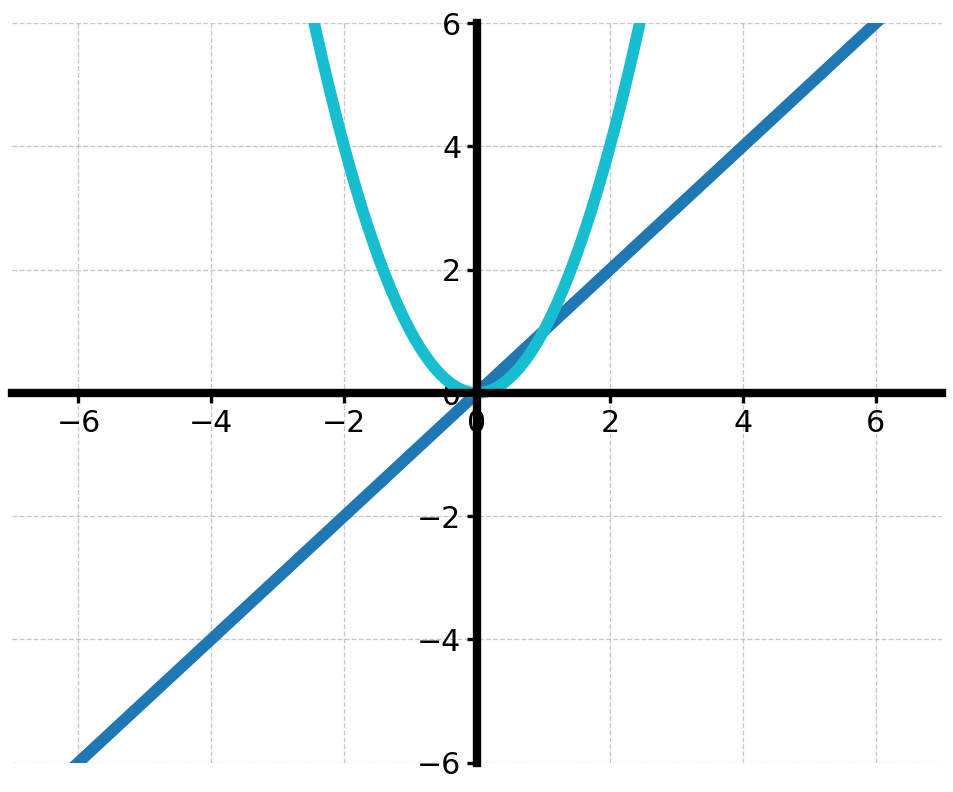
\includegraphics[scale = 0.35]{y__=__1x_and_y__=__x_power_2}}
\choice{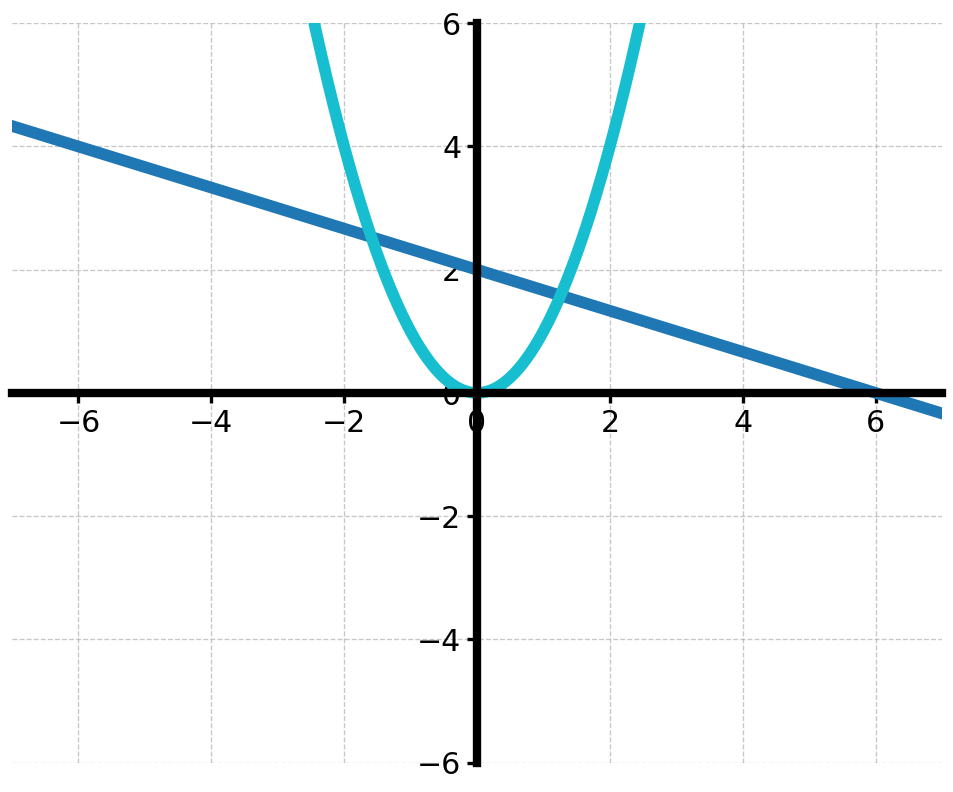
\includegraphics[scale = 0.35]{y__=___-_0.3333x__+__2_and_y__=__x_power_2}}
\choice{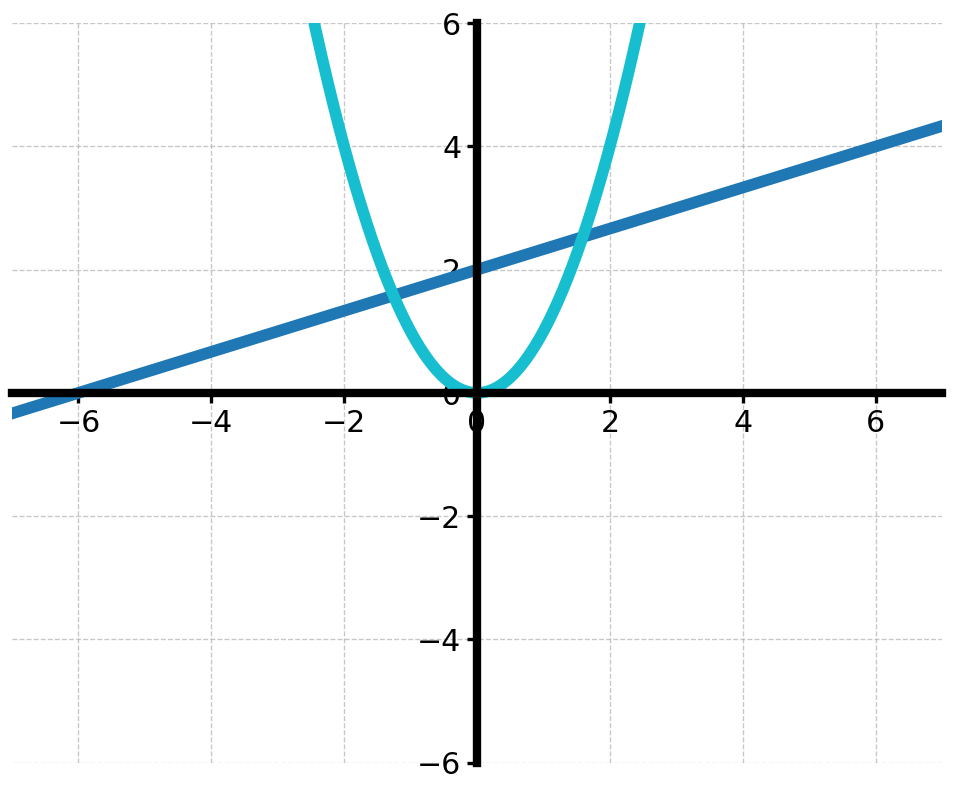
\includegraphics[scale = 0.35]{y__=___+_0.3333x__+__2_and_y__=__x_power_2}}
\end{fourchoice}

            }\question[1]{%
جواب‌های معادله $x^2 - 6 = 0$ در کدام گزینه وجود دارد؟.
    \begin{fourchoice}[4]\choice{$\sqrt{6}$ و $\sqrt{-6}$}
\choice{$\sqrt{6}$ و $-\sqrt{6}$}
\choice{$\sqrt{-36}$ و $\sqrt{36}$}
\choice{$\sqrt{0}$ و $\sqrt{36}$}
\end{fourchoice}

            }\question[2.5]{%
معادله $x^2 -2x = 0$ را به کمک روش هندسی حل کنید.‌
\\‌
\\‌
\\‌
\\‌
\\‌
\\‌
\\}\question[3]{%
اگر جمع دو عدد 3 و ضرب آنها -10 باشد، این دو عدد چه اعدادی هستند؟ راهنمایی باید معادله $x^2 -3x -10$ را حل کنید.‌
\\‌
\\‌
\\‌
\\‌
\\‌
\\}\question[1.5]{%
از معادله $2(x+y)=100$ مقدار x را بر حسب y محاسبه کنید.‌
\\‌
\\‌
\\‌
\\}\end{questions}
    \end{document}
    